\documentclass[landscape, 11pt]{report}

% Packages
\usepackage[landscape]{geometry}
\usepackage{amsmath}
\usepackage{xcolor}
\usepackage[utf8]{inputenc}
\usepackage[russian]{babel}
\usepackage{geometry}
\usepackage{graphicx}

% Options
\graphicspath{ {../figures/} {./figures/}}
\geometry{left=2.5cm,right=2.5cm,top=2.5cm,bottom=2.5cm}
\setlength\parindent{0pt}

% Title
\title{
	
\includegraphics[scale=0.07]{logo}\\
	\vspace{0.5em}
	Языки программирования. Семантика и система типов\\
	\vspace{0.2em}
	\Large Теоретическое задание. Тема 11
}
\author{Бронников Егор}
\date{}


\begin{document}
	
	% Титул
	
	\maketitle
	
	\vspace{-0.5cm}
	\hrule
	\vspace{0.5cm}
	
	% Задание 1
	
	\textbf{Задание 1.} Предположите правила типизации на основе ограничений для пар и типов-сумм. Используя предложенные правила, постройте дерево вывода типа с ограничениями, имеющее заключение:
	
	\begin{center}
		$. \quad \vdash \quad \lambda x : X . \, (case \; x \; of \; inl \, y \Rightarrow y \; | \; inr \, z \Rightarrow z.1).2 \; false \quad : \quad S \; |_{\chi} \; C$
	\end{center}
	
	для некоторых $S$, $C$ и $\chi$.
	
	\vspace{0.2cm}

	\textit{Решение.}
	
	\vspace{0.2cm}
	
	\textit{Правила типизации на основе ограничений для пар.}
	
	\vspace{0.2cm}
	
	$\dfrac{\Gamma \vdash t_1 : T_1 \; |_{x_1} \; C_1 \quad \Gamma \vdash t_2 : T_2 \; |_{x_2} \; C_2}{\Gamma \vdash \{t_1, t_2\} : T_1 \times T_2 \; |_{x} \; C_1 \cup C_2} \quad T\textup{-}Pair$
	
	\vspace{0.15cm}
	
	$\dfrac{\Gamma \vdash t : T \; |_{x} \; C}{\Gamma \vdash t.1 : T_1 \; |_x \; C \cup \{T = T_1 + T_2\}} \quad T\textup{-}Proj1$
	
	\vspace{0.15cm}

	$\dfrac{\Gamma \vdash t : T \; |_{x} \; C}{\Gamma \vdash t.2 : T_2 \; |_x \; C \cup \{T = T_1 + T_2\}} \quad T\textup{-}Proj2$

	\vspace{0.25cm}

	\textit{Правила типизации на основе ограничений для типов-сумм.}

	\vspace{0.2cm}

	$\dfrac{\Gamma \vdash t : T_1 \; |_{x} \; C}{\Gamma \vdash inl \; t : T_1 + T_2 \; |_x \; C} \quad T\textup{-}Inl$

	\vspace{0.15cm}
	
	$\dfrac{\Gamma \vdash t : T_2 \; |_{x} \; C}{\Gamma \vdash inr \; t : T_1 + T_2 \; |_x \; C} \quad T\textup{-}Inr$

	\vspace{0.15cm}

	$\dfrac{\Gamma \vdash t_0 : T \; |_{x} \; C_0 \quad \Gamma, x : T_1 \vdash t : X \; |_x \; C_1 \quad \Gamma, x_2 : T_2 \vdash t : Y \; |_x \; C_2}{\Gamma \vdash case \; t_0 \; of \; inl \, x_1 \Rightarrow t_1 \; | \; inr \, x_2 \Rightarrow t_2 : X \; |_x \; C_0 \cup C_1 \cup C_2 \cup \{X = Y, T = T_1 + T_2\}} \quad T\textup{-}Case$
	
	\vspace{0.25cm}
	
	\textit{Дерево вывода типа с ограничениями.}
	
	\begin{center}
		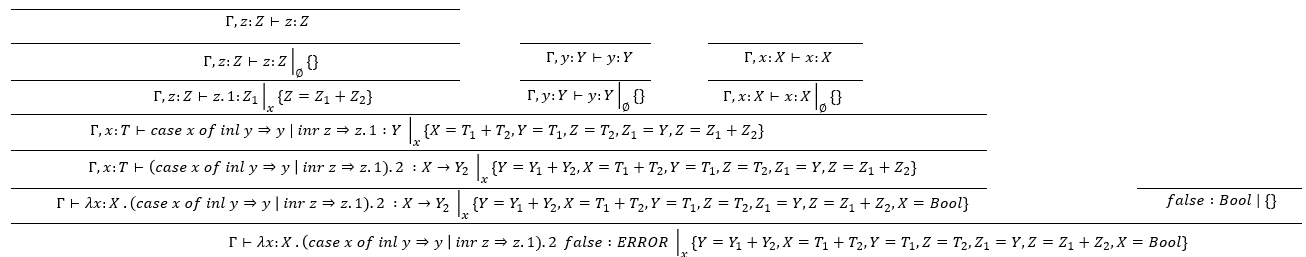
\includegraphics[scale=0.45]{solution}
	\end{center}
	
	\textit{Ответ.} Конфликт $\{X = T_1 + T_2, X = Bool\}$
	
	\vspace{0.1cm}
	\hrule
	
	\newpage
	
	% Задание 2
	
	\hrule
	\vspace{0.5cm}
	
	\textbf{Задание 2.} Выпишите главные унификаторы для следующих множеств ограничений, если возможно. Иначе, укажите ограничение, на котором алгоритм унификации выдаёт неудачу.
	
	\begin{itemize}
		\item[] \textit{(a)} $\{A \rightarrow B = B \rightarrow Nat, C \rightarrow A = Bool \rightarrow B\}$
		\item[] \textit{(b)} $\{A \rightarrow B = (C \rightarrow D) \rightarrow A, C \rightarrow A = B\}$
		\item[] \textit{(c)} $\{A = B \rightarrow B, C \rightarrow C = A \rightarrow B\}$
		\item[] \textit{(d)} $\{A \rightarrow B = B \rightarrow C, C \rightarrow A = A \rightarrow B\}$
		\item[] \textit{(e)} $\{A \rightarrow A = (B \rightarrow B) \rightarrow A, B \rightarrow A = (C \rightarrow C) \rightarrow (B \rightarrow B), C = D \rightarrow D\}$
	\end{itemize}
	
	\textit{Решение.}	
	
	\vspace{0.2cm}
	
	Главные унификаторы:
	
	\begin{itemize}
		\item[] \textit{(a)} $\{A = Nat, B = Nat, C = Bool\}$
		\item[] \textit{(b)} $\{B =A, C \rightarrow A = B\}$
		\item[] \textit{(c)} $\{A = B \rightarrow B, C = A, C = B\}$
		\item[] \textit{(d)} $\{A = B, B = C\}$
		\item[] \textit{(e)} $\{A = \left((D \rightarrow D) \rightarrow (D \rightarrow D)\right) \rightarrow \left((D \rightarrow D) \rightarrow (D \rightarrow D)\right), B = (D \rightarrow D) \rightarrow (D \rightarrow D), C = D \rightarrow D\}$
	\end{itemize}
	
	\hrule
	\vspace{0.5cm}
	
	% Задание 3
	
	\textbf{Задание 3.} Покажите, что следующие подстановки $\sigma$ и $\theta$ эквивалентны (т.е. $\sigma \sqsubseteq \theta$ и $\theta \sqsubseteq \sigma$):
	
	\vspace{-0.5cm}
	
	\begin{align*}
		& \sigma = [A \mapsto B, B \mapsto A \to Bool, C \mapsto A] \\
		& \theta = [B \mapsto C \to Bool]
	\end{align*}
	
	\newpage
	
	\textit{Решение.}
	
	\vspace{0.2cm}
	
	Необходимо рассмотреть применение подстановок $\sigma$ и $\theta$ к каждой из типов $A$, $B$ и $C$.
	
	\vspace{0.15cm}
	
	\textit{(a) Тип A.}
	
	\vspace{0.15cm}
	
	Применим подстановку $\sigma$ к типу $A$: $\sigma(A) = B$; $\sigma(B) = A \rightarrow Bool$, значит $\sigma(A) = A \rightarrow Bool$.
	
	Применим подстановку $\theta$ к типу $A$: $\theta(A) = A$.
	
	\vspace{0.2cm}
	
	\textit{(b) Тип B.}
	
	\vspace{0.15cm}
	
	Применим подстановку $\sigma$ к типу $B$: $\sigma(B) = A \rightarrow Bool$.
	
	Применим подстановку $\theta$ к типу $B$: $\theta(B) = C \rightarrow Bool$, так как $\sigma(C) = A$, то $\theta(B) = A \rightarrow Bool$.
	
	\vspace{0.2cm}
	
	\textit{(c) Тип C.}
	
	\vspace{0.15cm}
	
	Применим подстановку $\sigma$ к типу $C$: $\sigma(C) = A$; $\sigma(A) = B$, $\sigma(B) = A \rightarrow Bool$, значит $\sigma(C) = A \rightarrow Bool$.
	
	Применим подстановку $\theta$ к типу $C$: $\theta(C) = C$.
	
	\vspace{0.2cm}
	
	\textit{Ответ.} Подстановки $\sigma$ и $\theta$ -- не эквиваленты, так как $\sigma(A) = \sigma(B) = \sigma(C) = A \rightarrow Bool$, однако $\theta(A) = A$ и $\theta(C) = C$, то есть $\theta$ не меняется $A$ и $C$.

	\vspace{0.5cm}
	\hrule
	\vspace{0.5cm}
	
	% Задание 4
	
	\textbf{Задание 4.} Используя неявные аннотации типа и \verb|let|-полиморфизм, постройте дерево вывода типа с ограничениями и найдите главный тип для следующего выражения (в пустом контексте):
	
	\begin{center}
		$let \; f = \lambda s . \, \lambda z . \, s (s (s z)) \; in \, f \, f \, f$
	\end{center}

	\textit{Решение.}
	
	\vspace{0.5cm}
	
	\begin{center}
		$-$
	\end{center}
	
	\vspace{0.5cm}
	\hrule
	
\end{document}
